\chapter{Fudamentos Teóricos}\label{chapter:state-of-the-art}

El estudio del comportamiento de las trayectorias de movilidad humana a partir de datos de telefonía móvil ha cobrado gran relevancia en los últimos años debido a su potencial para abordar problemas complejos en áreas como la planificación urbana, la gestión del tráfico y la respuesta a emergencias. Sin embargo, la reconstrucción precisa de trayectorias a partir de registros de telefonía móvil presenta desafíos significativos, derivados de la naturaleza discreta, ruidosa y escasa de estos datos. En este capítulo, se realiza una revisión exhaustiva del estado del arte en torno a las técnicas de reconstrucción de trayectorias, las características de los datos de telefonía móvil y su aplicación en contextos específicos, con especial atención a las particularidades del caso cubano.

\section{Técnicas de completamiento de trayectorias}

El completamiento de trayectorias es un desafío multidimensional que combina técnicas clásicas y avanzadas para abordar la naturaleza fragmentaria de los datos de movilidad. A continuación, se analizan los enfoques existentes y sus implicaciones.

Las técnicas de interpolación lineal o \textit{splines} ofrecen simplicidad computacional pero requieren alta densidad de datos para garantizar precisión, una condición rara vez cumplida en registros de telefonía móvil \cite{hoteit2014estimating}. Para superar esto, enfoques como los de Vanemuise St. y Vajakas et al. integran restricciones de redes de tránsito, mapeando trayectorias al camino más corto o rápido entre puntos conocidos \cite{st2014reconstructing, vajakas2015trajectory}. Estos métodos priorizan la coherencia topológica pero pueden ignorar patrones de movilidad realista.

Técnicas de agrupamiento identifican patrones recurrentes en datos históricos para inferir trayectorias faltantes. Por ejemplo, Partsinevelos et al. combinan \textit{clustering} con redes neuronales para reconstruir trayectorias a partir de imágenes \cite{partsinevelos2005reconstructing}. En el ámbito probabilístico, las cadenas de Markov y redes bayesianas modelan transiciones entre estados espaciales, útiles para predecir rutas probables en contextos estructurados \cite{wang2016trajectory, jiang2022vehicle}. Chen et al. \cite{chen2019complete} aprovechan la regularidad en movilidad humana mediante factorización de tensores, ideal para completar trayectorias individuales con datos longitudinales. En telecomunicaciones, enfoques como los de Forghani et al. \cite{forghani2020cellular} y Derrmann et al. \cite{derrmann2019road} hibridizan datos de localización con información topológica o de \textit{handover} \footnote{El \textit{handover} entre torres es el proceso mediante el cual un dispositivo móvil cambia su conexión de una torre de telecomunicaciones a otra sin perder la comunicación. Esto ocurre cuando un usuario en movimiento se aleja de la torre a la que está conectado y entra en el rango de otra torre con una señal más fuerte o estable.} entre torres, demostrando aplicabilidad en entornos de baja resolución.

El marco GRFTrajRec \cite{zhaograph} ejemplifica técnicas modernas al emplear grafos espaciotemporales y modelos seq2seq para reconstruir trayectorias urbanas de baja frecuencia, permitiendo capturar atributos esenciales en cada punto y restaurar puntos GPS ausentes con alta precisión. De manera similar, Zhang et al. \cite{zhang2019prnet} combinan redes convolucionales, secuenciales y mecanismos de atención para estimar ubicaciones a partir de señales de telecomunicaciones, integrando posteriormente un emparejamiento de mapas para alinear las estimaciones con la red urbana \cite{zheng2014urban}. Estos métodos han demostrado ser efectivos para superar las limitaciones impuestas por la baja densidad de datos; sin embargo, suelen requerir grandes volúmenes de entrenamiento y una extensa preparación de datos.

En el ámbito del modelado secuencial, las redes recurrentes (\textit{Recurrent Neuronal Networks}, RNNs), y en particular sus variantes LSTM (Long Short-Term Memory), se destacan por su capacidad para capturar dependencias temporales gracias a un mecanismo que actualiza de forma continua el estado oculto a lo largo del tiempo \cite{elman1990finding}. En aplicaciones de movilidad, las LSTM permiten modelar la evolución del movimiento y estimar puntos ausentes basándose en información histórica \cite{manh2018scene, altche2017lstm}. No obstante, cuando se enfrentan a secuencias extensas o datos con grandes intervalos entre registros, su efectividad se ve limitada, pese a los mecanismos implementados para mitigar el desvanecimiento del gradiente \cite{hochreiter1991untersuchungen}.

Para abordar esto, los \textit{transformers} \cite{vaswani2017attention} han emergido como un paradigma disruptivo al sustituir la recurrencia por mecanismos de autoatención que ponderan dinámicamente todas las posiciones en una secuencia. En el contexto de la reconstrucción de trayectorias, arquitecturas como TrajBERT \cite{si2023trajbert} llevan este enfoque un paso más allá. TrajBERT extiende el modelo BERT \cite{devlin2018bert} al incorporar codificaciones posicionales que integran simultáneamente información espacial y temporal, lo que le permite capturar dependencias de largo alcance y correlaciones cruzadas entre puntos distantes, incluso cuando los datos son fragmentados o escasos.

En resumen, los métodos clásicos destacan por su simplicidad computacional y escalabilidad en entornos estructurados, aunque su precisión decae significativamente ante datos dispersos o patrones de movimiento no lineales. En contraste, los enfoques avanzados basados en aprendizaje automático, pese a requerir mayores recursos de entrenamiento y capacidad computacional, superan estas limitaciones al modelar relaciones complejas en los datos, ofreciendo mayor robustez en escenarios de alta dimensionalidad y tolerancia a variaciones en la calidad de los registros.

\section{Características y desafíos de los datos de telefonía móvil}

El crecimiento sostenido de la población humana, junto con su concentración en áreas urbanas y el aumento de su movilidad, ha planteado retos significativos para la adaptación de los sistemas sociales y demográficos. Estas dinámicas impactan directamente en la planificación y desarrollo de políticas públicas, ya que entender los patrones de movilidad resulta crucial para abordar problemas en diversas áreas. Por ejemplo, en la planificación del transporte, conocer cómo se desplazan las personas permite diseñar redes de carreteras más eficientes y sistemas de transporte público mejor adaptados a las necesidades de la población. En el ámbito de la salud, el modelado de la propagación de enfermedades infecciosas se beneficia de estos datos, ya que facilita la implementación de restricciones y controles más efectivos. Además, en el sector comercial, el marketing geográfico utiliza los patrones de movilidad para optimizar la distribución geográfica de publicidad y anuncios, maximizando su impacto \cite{asgari2013survey}.

Históricamente, el análisis de la movilidad humana se basaba en métodos tradicionales como encuestas, observación directa o censos poblacionales. Aunque útiles, estos enfoques presentan limitaciones significativas debido a su elevado costo, frecuencia limitada y dependencia de muestras pequeñas, lo que dificulta obtener una visión integral de los flujos de movilidad \cite{asgari2013survey}. En las últimas décadas, el desarrollo tecnológico ha permitido explorar nuevas fuentes de datos. Algunos estudios hacen uso de los sistemas GPS, que ofrecen una alta precisión en exteriores \cite{gong2012gps}; sin embargo, su uso puede ser intermitente debido al consumo de batería de los dispositivos, y por lo general requieren de la instalación de software específico y la activación del mismo por parte del usuario. Esto implica que los estudios basados en GPS suelan estar limitados a pequeñas muestras. Una alternativa, menos precisa pero mucho más abarcadora, es el uso de datos provenientes de las redes de telecomunicaciones, en particular los registros generados por los teléfonos móviles. Estos dispositivos, que actualmente son utilizados por el 80$\%$ de la población mundial mayor de 10 años y hasta el 90$\%$ en regiones como América y Europa \cite{ITU2024}, recopilan una cantidad masiva de datos vinculados a la actividad de sus usuarios \cite{toole2015path} que se requieren para el correcto funcionamiento de la red.

Los registros de telefonía móvil incluyen información como la identificación anónima del usuario, la ubicación de las radio bases con las que interactúan sus dispositivos y marcas temporales, permitiendo rastrear trayectorias de movilidad en tiempo real. Esto convierte a los teléfonos móviles en una plataforma de censado masivo de la actividad humana \cite{doyle2014population}, que no solo es económica y escalable, sino también capaz de proporcionar una visión general de los desplazamientos individuales y colectivos. Estas trayectorias ofrecen información valiosa para el análisis de la movilidad humana, contribuyendo a la toma de decisiones en múltiples campos y representando un recurso crucial para la investigación y el desarrollo de soluciones basadas en datos.

\subsection{Registros de telefonía móvil}

Una red de telefonía celular se compone de una infraestructura de radio desplegada en áreas denominadas celdas, cada una equipada con al menos una estación base transmisora-receptora fija (\textit{base transceiver station}, BTS) \cite{sharma2012cell}. Estas estaciones permiten establecer conexiones inalámbricas entre los terminales de los usuarios y la red en cualquier momento. Las interacciones generadas entre los dispositivos móviles y las BTS se almacenan en registros que contienen información clave, como identificadores de los usuarios y de las estaciones a las que se conectan \cite{yuan2013characterizing}. La estructura y el tipo de registros generados pueden variar según la tecnología utilizada por el proveedor de la red, aunque ciertos estándares han sido adoptados de manera general \cite{durive2021sistema}.

Entre los registros de mayor interés para estudios de movilidad se encuentran los registros detallados de llamadas (\textit{Call Detail Records}, CDR) y los registros de actualización de área (\textit{Location Area Update}, LAU) \cite{gutierrez2020como}. Los CDR se generan durante eventos específicos, como llamadas, mensajes o conexiones a la red, y son comúnmente utilizados para la facturación de los usuarios, lo que asegura su almacenamiento por largos períodos. Estos registros incluyen información como identificadores de los dispositivos, marcas de tiempo y tipos de eventos, siendo ampliamente utilizados en estudios de movilidad gracias a su disponibilidad. Por otro lado, los LAU son activados por la red en situaciones como cambios de cobertura o períodos de inactividad, proporcionando una mayor resolución temporal al registrar eventos independientes de las actividades de los usuarios. Sin embargo, debido a que no son utilizados para facturación, suelen ser desechados, lo que limita su aplicación en estudios de movilidad \cite{durive2021sistema}.

A pesar de las diferencias en los eventos que generan estos registros, ambos comparten una estructura de información similar, incluyendo identificadores, eventos, celdas y marcas temporales. Estos datos permiten aproximar las localizaciones de los usuarios en diferentes momentos, aunque la resolución espacial depende de la densidad de las BTS, la cual varía significativamente entre áreas urbanas y rurales \cite{forghani2020cellular}. Al identificar registros con el mismo identificador de usuario, es posible reconstruir trayectorias aproximadas que muestran las posiciones de las estaciones base a las que un dispositivo se conectó mientras se desplazaba \cite{chen2018individual}. En este contexto, una colección de trayectorias derivadas de datos de telefonía móvil puede ofrecer una representación aproximada de la movilidad.

\subsection{Desafíos}

Los datos de redes de telecomunicaciones han revolucionado los estudios de movilidad humana al proporcionar grandes volúmenes de información que superan las limitaciones de métodos tradicionales como las encuestas. Aunque estos datos han abierto nuevas posibilidades para investigar patrones de movilidad, también presentan desafíos significativos.

Uno de los principales retos es garantizar la privacidad de los usuarios, lo que ha llevado a restringir el acceso a los registros, incluso cuando se encuentran anonimizados. Por esta razón, una tendencia emergente en la literatura es la construcción de modelos que capturan aspectos de la movilidad y permiten compartir información sin que las limitaciones de privacidad impidan su desarrollo. Por ejemplo en \cite{tesselkin2017estimation} se presenta un modelo de red de transporte en forma de cadena de Markov para la estimación de las matrices origen-destino (O-D). Con cierta similitud, en \cite{pourmoradnasseri2019od} un modelo de Markov de segundo orden es empleado bajo la premisa de investigar patrones de movilidad humana a partir de telefonía celular.

La naturaleza masiva y en tiempo real de los datos generados por las redes de telecomunicaciones impone una gran presión sobre las infraestructuras de procesamiento y almacenamiento. El reto de la escalabilidad no solo se refiere a la capacidad de almacenar grandes volúmenes de datos, sino también a la necesidad de desarrollar algoritmos y sistemas que permitan procesarlos de manera eficiente y en tiempos adecuados. En este contexto, la adopción de arquitecturas de procesamiento distribuido ha sido fundamental. Herramientas y frameworks como Apache Hadoop y Apache Spark han demostrado ser eficaces para abordar estos problemas, permitiendo la ejecución de tareas de análisis y minería de datos en entornos paralelos y de alta disponibilidad \cite{zaharia2016apache}. Sin embargo, la implementación de estas soluciones implica desafíos adicionales, como la optimización de la asignación de recursos y la gestión de la latencia en el procesamiento de datos en tiempo real.

Otro desafío importante es la integración de los registros de telefonía con otras fuentes de información, tales como mapas digitales, datos de sensores ambientales y sistemas de monitoreo del tráfico. La combinación de estos datos heterogéneos tiene el potencial de enriquecer el análisis de la movilidad, permitiendo la validación cruzada de modelos y ofreciendo una visión más completa y contextualizada del entorno urbano. No obstante, la integración de datos provenientes de distintas fuentes requiere el desarrollo de metodologías robustas para asegurar la coherencia y la sincronización tanto a nivel espacial como temporal. Problemas relacionados con la estandarización de formatos, la calidad y la resolución de los datos son comunes en estos escenarios. Algunos estudios han explorado enfoques para la fusión de datos que buscan mitigar estas dificultades, demostrando mejoras significativas en la precisión y la fiabilidad de las estimaciones de movilidad \cite{batty2012smart}. La implementación de estos enfoques demanda, además, la creación de protocolos y herramientas específicas que faciliten la interoperabilidad entre sistemas y garanticen una integración efectiva.

A pesar de los avances en el procesamiento y análisis de datos basados en registros de telefonía, el balance entre el aprovechamiento de la información, la protección de la privacidad, la escalabilidad y la integración con otras fuentes sigue siendo una barrera crítica en la investigación. En contextos donde el acceso a datos es fundamental para obtener resultados significativos, superar estos desafíos representa un paso esencial para el desarrollo de modelos cada vez más precisos y aplicables a la planificación y gestión urbana.

\section{Datos de telefonía móvil en Cuba}

La Empresa de Telecomunicaciones de Cuba, ETECSA, es la única empresa en el territorio nacional que provee servicios de telefonía móvil e Internet. A pesar de grandes avances los últimos años, estos servicios demoraron más tiempo para hacerse populares y accesibles a la mayor parte de la población cubana respecto a la media mundial \cite{durive2021sistema}. Como consecuencia directa, la experiencia con el uso de datos de la red de telefonía celular para estudios de movilidad en Cuba está limitada a años recientes.

En 2018 comienza un esfuerzo por parte de investigadores del actual Centro de Sistemas Complejos de la Facultad de Física de la Universidad de La Habana para acceder a los registros de telefonía celular \cite{durive2021sistema}, con el objetivo de extraer analítica que enriqueciera los procesos de toma de decisiones por parte de las autoridades de salud, planificación del transporte y estudios socio-demográficos, etc. Obteniéndose el acceso a registros de tipo LAU a partir del año 2020, acordándose con ETECSA la firma de un acuerdo de confidencialidad con la universidad y el compromiso de respetar una serie de métodos de seguridad entre los que figura que:

\begin{itemize}
    \item los datos de LAU son almacenados en servidores de ETECSA, dentro de la red de la compañía;
    \item los datos son almacenados sin identificadores de usuarios, como nombre, teléfono o IMSI;
    \item ningún dato de granularidad individual puede sustraerse de la red de la empresa;
    \item ningún procedimiento de ingeniera inversa o \textit{de-anonymization} puede usarse;
    \item los datos se entregan con fines de investigación y solo pueden usarse para estos fines;
    \item ETECSA emite por escrito autorización para la divulgación de los resultados obtenidos.
\end{itemize}

ETECSA ha desplegado más de 1,500 radiobases en Cuba, con una distribución heterogénea que refleja la densidad de usuarios, concentrándose en áreas urbanas. Para proteger la ubicación precisa de estas torres, se adoptó una estrategia que agrupa torres cercanas en zonas densas y ajusta ligeramente su posición en zonas rurales, reduciendo el número a 795 pseudo-torres con ubicaciones GPS compartidas. Estas pseudo-torres se emplean en estudios de movilidad mediante zonas de cobertura definidas con celdas de Voronoi, funcionando de manera similar a las torres reales para los análisis realizados.

El estudio de la movilidad poblacional a partir de los registros LAU de la empresa ETECSA está amparado por la legislación cubana. En particular la Ley de protección de Datos Personales \cite{cuervo2022resolucion}, del 2022, define lo que se consideran datos personales (que incluye los datos generados por sistemas tecnológicos como los teléfonos) y las reglas para su uso. Estipula que dichos datos pueden usarse por razones de bienestar general si se someten previamente a un procedimiento de disociación, como el antes mencionado.

El valor social de comprender y usar estos datos quedó demostrado ampliamente cuando, en medio de la pandemia de SARS-CoV-2 a partir de marzo de 2020, el sistema de salud y el gobierno cubanos pudieron disponer de modelos de movilidad para evaluar la efectividad de las medidas de limitación de movimiento que se implementaron. Es importante resaltar que, durante ese mismo período, la mayor parte de los gobiernos del mundo usaron métricas semejantes para entender la epidemia y sus consecuencias \cite{sulyok2020community, saha2020lockdown, nanda2022community, hakim2021mitigation}. En muchos casos, los modelos de movilidad provinieron de empresas como Google que, amparada por la urgencia médica mundial, puso a disposición de los investigadores modelos de movilidad basados en la detección de posicionamiento de los usuarios a partir de los metadatos generados por sus aplicaciones \cite{Google2020Mobility}. Es de señalar que Google excluyó a Cuba de la lista de países que podían acceder a dichos datos, como se muestra en la figura \ref{fig:google_exclusion}.

\begin{figure}[!htb] 
    \centering 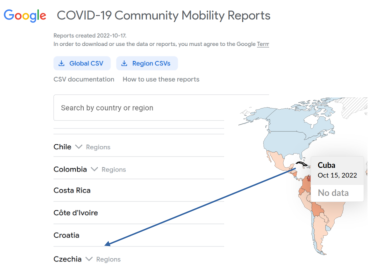
\includegraphics[width=1\textwidth]{Graphics/google_exclusion.pdf} \caption{Cuba excluida por Google en el acceso a modelos de movilidad} \label{fig:google_exclusion}
\end{figure}

Si bien los modelos de movilidad generados por el Centro de Sistemas Complejos, de acuerdo con ETECSA, fueron de gran utilidad, es importante señalar que dichos datos tienen menos precisión y son menos abundantes que los que disponen empresas como Google, Facebook y otras.

Una de las enseñanzas de la pandemia y de la posterior aplicación de estos datos al estudio de la movilidad poblacional es que no se puede esperar a tener situaciones críticas para decidirse a usar estos métodos de análisis de datos. Esencialmente, aunque el posible uso y valor de estos datos sea bastante obvio, en los detalles de cómo extraer valor informacional radica un gran reto. Es importante crear una base científica y tecnológica que permita, ante necesidades concretas, saber las potencialidades de estos datos, si permiten o no enfrentar la tarea en cuestión, y la precisión de los mismos.

\subsection{Estudios cubanos relacionados}

La investigación en Cuba sobre el uso de datos de telefonía móvil para análisis de movilidad y aplicaciones epidemiológicas ha experimentado avances significativos en los últimos años. Roger \cite{casimiro2019movilidad} sentó las bases al desarrollar un sistema informático para procesar registros de llamadas en colaboración con ETECSA, generando matrices origen-destino a escala nacional y demostrando su utilidad en modelación de epidemias. Posteriormente, Orlando \cite{durive2021sistema} profundizó en la extracción de indicadores de movilidad mediante herramientas de inteligencia artificial, desarrollando el \textit{software} BDPhoneFlow, y analizó el impacto de las medidas sanitarias durante la COVID-19. Lius Padrón \cite{padron2021transporte} validó el uso de datos de LAU para identificar disparidades temporales en flujos de movilidad, destacando el efecto del escalonamiento de horarios como medida socioeconómica.

En el ámbito epidemiológico, Alejandro Castro \cite{castro2023movilidad} exploró la relación entre matrices de movilidad derivadas de telefonía y casos de COVID-19 en La Habana, revelando limitaciones en la predictibilidad debido a la preponderancia de contagios intra-área. Por su parte, Andy \cite{rodriguez2022movilidad} abordó específicamente el completamiento de puntos intermedios en trayectorias mediante un modelo de redes neuronales, implementando experimentos en entornos urbanos artificiales y extendiendo su aplicación a datos reales de La Habana. Ernesto \cite{ortega2022modelacion} complementó estos esfuerzos con modelos de física estadística, evaluando la eficacia del rastreo de contactos en Cuba durante la pandemia y destacando el papel crítico de las pruebas masivas.

Aunque estos trabajos han establecido metodologías valiosas, aún existen varios desafíos pendientes, entre ellos el completamiento preciso de trayectorias individuales integrando patrones espaciotemporales complejos en modelos predictivos. Estas limitaciones resaltan la necesidad de enfoques innovadores que combinen el conocimiento local con arquitecturas avanzadas de aprendizaje automático.

\section{Contribución de esta investigación}

Esta investigación propone la aplicación de TrajBERT para el completamiento de trayectorias a partir de datos de telefonía móvil en Cuba. A diferencia de trabajos anteriores que priorizaron el análisis estadístico sobre patrones de movilidad colectiva (matrices origen-destino), esta tesis se centra en reconstruir trayectorias a nivel de usuario individual, un desafío técnicamente más complejo y menos explorado en Cuba. TrajBERT se orienta al completamiento de trayectorias implícitas sin requerir información adicional, como velocidad, condiciones climáticas u otras variables contextuales. Estas características coinciden con la naturaleza de los registros de telefonía en Cuba, lo que hace que este modelo resulte especialmente idóneo para su aplicación en dicho contexto.

Al aplicar una arquitectura basada en \textit{transformers}, se espera superar la efectividad del estudio previo basado en redes neuronales tradicionales \cite{rodriguez2022movilidad}, al tratar las trayectorias como secuencias de ubicaciones interrelacionadas en el espacio y el tiempo, logrando una comprensión más exacta de los patrones de movilidad. Este enfoque promete captar de manera más precisa las dependencias espaciotemporales, posibilitando un completamiento robusto incluso en escenarios con datos escasos y de baja densidad.